\documentclass[a4paper,12pt,oneside]{report}

\usepackage[left=1.55in,right=1.15in,top=1in,bottom=1.15in]{geometry}
\usepackage{graphicx}
\usepackage{array}
\usepackage{booktabs}
\usepackage{longtable}
\usepackage{float}
\usepackage{enumitem}
\usepackage[table]{xcolor}
\usepackage{hyperref}

\hypersetup{
    colorlinks=true,
    linkcolor=blue,
    urlcolor=red,
    citecolor=green
}
\urlstyle{tt}

\setlist[itemize]{leftmargin=1.35em,topsep=4pt,itemsep=3pt,parsep=0pt,partopsep=0pt}
\setlist[enumerate]{leftmargin=1.6em,topsep=4pt,itemsep=4pt,parsep=0pt,partopsep=0pt}
\renewcommand{\arraystretch}{1.18}

\newcommand{\projectname}{Tactical Cards}
\newcommand{\groupname}{Group 2 (\projectname)}
\newcommand{\submissiondate}{TBC - confirm on Moodle}
\newcommand{\wcell}[2]{\parbox[t]{#1}{\raggedright #2}}
\newcommand{\code}[1]{\path{#1}}
\renewcommand{\bibname}{Reference}

\begin{document}

\begin{titlepage}
\begin{center}
\vspace*{20pt}

\includegraphics[width=0.55\textwidth]{../wr2-latex/nottingham-logo.png}\\[1cm]
\vspace{28pt}
{\Large\bfseries COMP4135 SEM Final Group Report}\\[18pt]
{\large\bfseries \groupname}\\[34pt]
{\large\bfseries Team members}\\[14pt]
Guangjun HU (20511787)\\
Hongshuo HU (20808603)\\
Cheng YE (20513323)\\
Zehan CHEN (20807750)\\[32pt]
School of Computer Science\\
University of Nottingham
\end{center}

\vfill
\begin{center}
\textbf{Submission Date: \submissiondate}
\end{center}
\end{titlepage}

\chapter*{Abstract}
\addcontentsline{toc}{chapter}{Abstract}
Tactical Cards is a Unity-based tactical card combat prototype designed for teenagers and casual strategy players who benefit from readable, small-scope decision making. The final project delivers a complete single-battle loop with a title screen, a playable tactical encounter on a grid board, a result screen, card-driven unit actions, deterministic enemy response, and a themed runtime HUD. Development was deliberately kept within a compact vertical slice so the team could prioritise maintainable code structure, automated validation, and visible teamwork evidence alongside gameplay implementation. The delivered project combines early requirements work from WR1, implementation and scope-control decisions from WR2, and a validation-heavy WR3 plus post-WR3 polish cycle. By the end of the project, the codebase had stable EditMode and PlayMode test coverage, a documented issue-closure trail, and a clearer UI/UX layer that addressed earlier feedback about readability, feedback, and onboarding.

\tableofcontents

\chapter{Introduction}

\projectname{} is a Unity-based tactical card battle prototype designed for teenagers and casual strategy players. The delivered software provides a complete single-battle session: the player enters through a start screen, controls allied units on a grid, plays tactical cards, observes enemy response, and reaches a clear result state.

\section{Motivation}

The project began from one simple design goal: each turn should ask the player to make a small number of visible and meaningful tactical decisions without requiring a large content set or a complicated ruleset. Instead of aiming for a campaign-heavy tactics game, the design focuses on one encounter in which positioning, range, timing, and action order matter.

The tactical card format was chosen because it combines two readable systems. First, a grid-based battle makes spatial decisions visible on screen. Second, a small hand of action cards introduces variety without turning the project into a deckbuilding or collection-heavy game. This makes the game strategically meaningful while still remaining approachable for the intended audience.

\section{Report Scope}

This report is written as a self-contained final software-engineering document rather than as a change log. The main chapters focus on the delivered system itself: background, requirements, development, validation, maintenance, and reflection. Supporting technical artifacts are preserved in the appendices, including the user manual, meeting minutes, representative test evidence, development planning notes, version-control summary, and document register.

That structure is deliberate. It allows the main discussion to stay focused on the product and the engineering decisions behind it, while still showing that the submission satisfies the wider expectations of a software-engineering project report: a concrete software artifact, updated system and UI design, traceable requirement evolution, implementation strategy, validation evidence, and reflective discussion of technical and team-level work \cite{courseSpecification}.

\section{Aims and Objectives}

The project has four main objectives.

\begin{enumerate}
    \item Deliver a complete playable battle loop in Unity, including player turn, enemy turn, and battle-end handling.
    \item Keep the gameplay narrow enough that the core interactions remain readable, stable, and testable.
    \item Build the system so that turn flow, card resolution, grid interaction, and runtime UI are understandable at code level.
    \item Improve interface clarity and feedback so that a first-time player can understand what to do without outside explanation.
\end{enumerate}

Success is therefore defined less by feature quantity than by the completeness of one polished vertical slice. A successful outcome means that a player can launch the game, start a battle, understand the interaction order, observe enemy response, finish the encounter, and then replay or return cleanly to the menu.

\section{Delivered Contribution}

The delivered build is intentionally modest in content, but complete in structure. It contains:

\begin{itemize}
    \item a full start-to-result session flow;
    \item a 6x6 tactical battle with card-driven actions and deterministic enemy response;
    \item a panel-based HUD with direct action feedback, prompts, and world-space health bars;
    \item automated validation for deterministic runtime behaviour, plus manual smoke for presentation-heavy UI;
    \item a code structure that separates flow, battle rules, UI, and presentation cleanly.
\end{itemize}

The project did not remain static from concept to completion. Early design assumptions were revised as playable builds exposed onboarding, readability, and session-flow problems. The report therefore does not present the final system as if it had emerged fully formed. Chapter 3 explains how the requirement set evolved from the earliest design baseline into the delivered implementation, and Chapter 4 explains how that evolution was handled through iterative development rather than a once-through sequence.

\chapter{Background and Related Work}

The delivered game sits in a recognisable design space between a small-scale tactical skirmish game and a card-driven command system. However, the project was never intended to compete with content-heavy strategy RPGs or large collectible card games. From the start, the team treated related work as a guide for framing interaction patterns rather than a source of gameplay scope inflation. That position is consistent with both the coursework brief and the early one-pager, which emphasised a readable, teenager-friendly tactical prototype rather than a broad commercial feature set \cite{cw1Specification,onePager}.

\section{Design Context}

The core design context was a lightweight tactical grid battle in which the player controls a very small team and spends a limited hand of cards each turn. This places \projectname{} closer to a command-oriented tactics prototype than to a deckbuilding game. Positioning, range, targeting, and action ordering are the main decision variables, while content breadth is intentionally constrained. The project therefore uses cards as a readable action language, not as a collectible system with large pools, rarity, or synergy chains \cite{onePager}.

Unity was selected because the game depends on both world-space interaction and screen-space feedback. The board, tile highlights, unit placement, and combat feedback all live in the same runtime environment as the HUD, menu flow, and result presentation. That makes Unity a better fit than a document-style prototype or a purely web-first interface for this coursework. It also allowed the team to demonstrate software-engineering concerns that matter for game development in practice, such as separating turn rules from view state, isolating assets, and validating behaviour across both scene logic and UI flow.

Just as importantly, the team chose to keep the product as one polished encounter rather than stretching toward multiple maps, progression systems, or a larger content pipeline. This was not simply a feature cut; it was a design decision to preserve clarity and testability. A compact battle loop gave the team enough room to implement and validate selection order, card resolution, enemy response, battle-end transitions, and usability refinements without diluting the engineering evidence with unfinished systems \cite{cw1Specification}.

\section{Reference Strategy}

The team used external references selectively and at two different levels. At the gameplay level, the project borrowed only broad genre patterns: grid occupancy, ranged versus melee positioning, and card-labelled actions. No external gameplay framework was imported into the runtime. The battle loop, flow coordination, grid logic, enemy response, and HUD behaviour were authored within the project codebase under the main runtime scripts, which keeps ownership boundaries clear and makes the resulting software easier to explain in the report.

At the asset level, the team deliberately adopted a `CC0-first` strategy during the post-WR3 visual pass so that the final package would remain easy to attribute and redistribute. The imported first-slice UI theme uses Kenney packs for panels, buttons, and icons, while later visual work fell back to team-authored presentation code for unit silhouettes and board dressing when a coherent local character pack was not yet ready for stable import \cite{postWr3OpenAssetRegister}. This distinction matters: the UI art is third-party and documented, but the presentation wiring, layout logic, and gameplay-facing behaviour remain original coursework implementation.

The main consequence of this reference strategy is that related work shaped form more than function. External material helped the team avoid placeholder visuals and supported a clearer tabletop-fantasy identity, but it did not replace the need for local engineering decisions. The delivered system is therefore best understood as an original tactical vertical slice built with carefully bounded reference use, not as an assembly of imported mechanics.

\section{Related-Work Boundary}

Because this is a coursework prototype rather than an academic game-studies paper, the related-work discussion remains intentionally practical. The most relevant comparison points are genre conventions and asset-source choices, not a long survey of published games. The report therefore focuses on the references that materially affected implementation: the initial design brief, the one-pager that constrained scope, and the open-licensed asset sources that informed the final presentation direction \cite{cw1Specification,onePager,postWr3OpenAssetRegister}.

\chapter{Requirements Engineering}

The requirements for \projectname{} were first established in WR1 and then refined as the team moved from concept definition to a stable vertical slice. The final requirement set preserves the original design intent of a readable tactical card game for teenagers, but it has been updated to reflect the actual delivered system rather than the earlier prototype-only view \cite{cw1Specification,onePager}.

\section{Requirements Elicitation}

Three stakeholder perspectives shaped the project requirements.

\begin{itemize}
    \item \textbf{Teenage end users.} The game needed to be understandable within a short session, readable on screen, and strategically meaningful without deep genre knowledge.
    \item \textbf{The teaching team and module assessor.} The project needed to show clear software-engineering practice, including requirements work, planning, testing, documentation, and teamwork evidence.
    \item \textbf{The development and maintenance perspective.} The implementation needed to remain small enough to build, test, debug, and explain within the coursework period.
\end{itemize}

Early elicitation work, including the one-pager and WR1 reporting, narrowed the project toward a lightweight tactical battle rather than a large campaign game. That decision was reinforced by early meetings, which made it clear that the team needed a scope that could support both gameplay delivery and a strong reportable engineering process. As a result, the team treated the project as a compact battle-simulation product rather than a content-heavy game.

\section{Requirements Specification}

Table \ref{tab:final-requirements} presents the final requirement set used for the completed system. The list combines the original WR1 requirements with the post-WR3 UI/UX completion work so that the specification matches the delivered game.

\begin{table}[H]
\centering
\small
\begin{tabular}{lll}
\toprule
\wcell{1.7cm}{\textbf{ID}} & \wcell{5.1cm}{\textbf{Requirement}} & \wcell{5.0cm}{\textbf{Delivered meaning in the final build}} \\
\midrule
\wcell{1.7cm}{FR-01} & \wcell{5.1cm}{The game shall provide a complete front-end flow.} & \wcell{5.0cm}{The player can move from title screen to battle and then to a result state with replay or return-to-menu actions.} \\
\wcell{1.7cm}{FR-02} & \wcell{5.1cm}{The game shall initialise one playable tactical battle on a small grid.} & \wcell{5.0cm}{The battle scene creates a 6x6 board, places player and enemy units, and starts a valid battle loop.} \\
\wcell{1.7cm}{FR-03} & \wcell{5.1cm}{The player turn shall refresh battle resources and draw a hand of cards.} & \wcell{5.0cm}{Turn start resets the playable-action budget and refreshes the runtime hand.} \\
\wcell{1.7cm}{FR-04} & \wcell{5.1cm}{The player shall be able to select a unit, choose a card, and act on a valid target only.} & \wcell{5.0cm}{The HUD and board flow enforce valid ordering and surface invalid-target feedback.} \\
\wcell{1.7cm}{FR-05} & \wcell{5.1cm}{Command cards shall support movement, attack, defence, repositioning, and recovery.} & \wcell{5.0cm}{The final card set includes Move, Dash, Strike, Long Strike, Guard, Push, and Recover.} \\
\wcell{1.7cm}{FR-06} & \wcell{5.1cm}{Enemy units shall execute visible and deterministic turns.} & \wcell{5.0cm}{Enemy AI targets the nearest valid player and either attacks or advances accordingly.} \\
\wcell{1.7cm}{FR-07} & \wcell{5.1cm}{The game shall expose clear victory and defeat states.} & \wcell{5.0cm}{Battle outcome transitions into a result panel with replay and menu actions.} \\
\wcell{1.7cm}{FR-08} & \wcell{5.1cm}{The runtime HUD shall expose the key battle state clearly.} & \wcell{5.0cm}{The final HUD shows prompts, hand, energy, battle log, card availability, and world-space health bars.} \\
\wcell{1.7cm}{NFR-01} & \wcell{5.1cm}{The game shall remain suitable for teenage users.} & \wcell{5.0cm}{The rules, UI flow, and feedback are intentionally kept compact and readable.} \\
\wcell{1.7cm}{NFR-02} & \wcell{5.1cm}{The project shall remain feasible within coursework scope.} & \wcell{5.0cm}{The team keeps to a single-battle vertical slice instead of expanding into campaign systems.} \\
\wcell{1.7cm}{NFR-03} & \wcell{5.1cm}{The implementation shall remain testable and maintainable.} & \wcell{5.0cm}{The codebase is modularised by responsibility and protected by EditMode and PlayMode tests.} \\
\wcell{1.7cm}{NFR-04} & \wcell{5.1cm}{Third-party assets and components shall be traceable.} & \wcell{5.0cm}{Imported UI art is recorded in asset notices and supporting registers.} \\
\wcell{1.7cm}{NFR-05} & \wcell{5.1cm}{The project shall remain documentable and traceable as coursework evidence.} & \wcell{5.0cm}{Milestones, tests, issue logs, and process records are archived under the project records tree.} \\
\bottomrule
\end{tabular}
\caption{Final functional and non-functional requirements for Tactical Cards.}
\label{tab:final-requirements}
\end{table}

\section{Requirements Validation}

The requirements were validated through a combination of direct automated tests, PlayMode smoke checks, manual visual smoke, and issue-driven iteration. This layered approach was necessary because the project contains both deterministic game rules and presentation-heavy UI concerns. Core systems such as turn flow, card resolution, grid occupancy, enemy behaviour, and game bootstrap were validated directly with automated tests. By contrast, visual layout questions such as title readability or hand-panel occlusion required manual smoke supported by targeted regression tests.

Table \ref{tab:requirements-validation-map} summarises how the main requirement groups were validated in the delivered project.

\begin{table}[H]
\centering
\small
\begin{tabular}{lll}
\toprule
\wcell{2.0cm}{\textbf{Requirement group}} & \wcell{4.6cm}{\textbf{Validation approach}} & \wcell{5.2cm}{\textbf{Primary evidence}} \\
\midrule
\wcell{2.0cm}{Battle bootstrap and flow} & \wcell{4.6cm}{EditMode bootstrap tests plus PlayMode smoke} & \wcell{5.2cm}{`GameRootTests`, `GameFlowControllerTests`, `BattleFlowPlayModeTests`} \\
\wcell{2.0cm}{Cards and turn loop} & \wcell{4.6cm}{EditMode rule-level tests} & \wcell{5.2cm}{`TurnManagerTests`, `DeckManagerTests`, `CardResolverTests`} \\
\wcell{2.0cm}{Grid and unit state} & \wcell{4.6cm}{EditMode placement, movement, damage, and occupancy tests} & \wcell{5.2cm}{`GridManagerTests`, `UnitControllerTests`, `TileViewTests`} \\
\wcell{2.0cm}{Enemy response} & \wcell{4.6cm}{EditMode AI tests plus turn-loop integration checks} & \wcell{5.2cm}{`EnemyAITests`, `TurnManagerTests`} \\
\wcell{2.0cm}{HUD and interaction feedback} & \wcell{4.6cm}{EditMode UI tests plus manual smoke for final layout} & \wcell{5.2cm}{`BattleUITests`, `CardButtonViewTests`, post-WR3 smoke records} \\
\wcell{2.0cm}{Usability refinements} & \wcell{4.6cm}{Heuristic walkthrough followed by post-WR3 issue closure and smoke retest} & \wcell{5.2cm}{WR2 walkthrough and post-WR3 issue log} \\
\bottomrule
\end{tabular}
\caption{How the final requirement groups were validated.}
\label{tab:requirements-validation-map}
\end{table}

This validation path also reflects how the requirements matured. Early heuristic feedback showed that onboarding clarity, enemy-phase readability, and battle-end presentation were still weak in the prototype. Those gaps later became explicit implementation and testing targets during the post-WR3 completion push. As a result, the final requirement set is not only an early design wish list; it is a refined specification backed by implementation and validation evidence.

\chapter{Development}

This chapter describes the architecture, implementation structure, runtime interaction model, simulation rules, UI design, and the iterative process used to deliver the final build.

\section{System Design}

The runtime architecture is split by responsibility rather than by scene object alone. This keeps the battle systems readable and makes it easier to test core behaviour directly.

\begin{figure}[H]
\centering

\includegraphics[width=0.93\textwidth]{architecture-diagram.png}
\caption{High-level runtime architecture for \projectname{}.}
\label{fig:architecture}
\end{figure}

This architecture diagram shows the major runtime modules and the direction of interaction between flow, board, cards, units, and UI. It communicates system responsibilities and runtime coordination at a level that a class-level inheritance diagram would not.

\begin{figure}[H]
\centering

\includegraphics[width=0.93\textwidth]{module-map.png}
\caption{Simplified module dependency and responsibility map.}
\label{fig:module-map}
\end{figure}

The module map complements the architecture view. The architecture diagram explains \textit{what} subsystems exist and how they interact; the module map explains \textit{where} those responsibilities live in the codebase. Table \ref{tab:runtime-components} extends those two figures with the final component inventory.

\begin{table}[H]
\centering
\small
\begin{tabular}{llll}
\toprule
\wcell{2.2cm}{\textbf{Area}} & \wcell{3.7cm}{\textbf{Key classes}} & \wcell{4.8cm}{\textbf{Responsibility}} & \wcell{1.8cm}{\textbf{Origin}} \\
\midrule
\wcell{2.2cm}{Core flow} & \wcell{3.7cm}{`GameRoot`, `GameFlowController`, `GameFlowState`, `TurnManager`} & \wcell{4.8cm}{Scene bootstrap, title-battle-result flow, battle session start, turn state, and win/loss resolution} & \wcell{1.8cm}{Group-authored} \\
\wcell{2.2cm}{Cards} & \wcell{3.7cm}{`CardData`, `DeckManager`, `CardResolver`} & \wcell{4.8cm}{Card definitions, deck lifecycle, draw/discard handling, and explicit effect resolution} & \wcell{1.8cm}{Group-authored} \\
\wcell{2.2cm}{Grid} & \wcell{3.7cm}{`GridManager`, `TileView`} & \wcell{4.8cm}{Board generation, occupancy, movement, range queries, and highlight state} & \wcell{1.8cm}{Group-authored} \\
\wcell{2.2cm}{Units} & \wcell{3.7cm}{`UnitController`, `EnemyAI`} & \wcell{4.8cm}{Shared unit state, damage/heal/guard behaviour, and deterministic enemy targeting and movement} & \wcell{1.8cm}{Group-authored} \\
\wcell{2.2cm}{Runtime HUD} & \wcell{3.7cm}{`BattleUI`, `BattleHudSnapshot`, `CardButtonView`, `UnitHealthBarView`} & \wcell{4.8cm}{Battle-state presentation, runtime card views, prompts, disabled-card feedback, and world-space health bars} & \wcell{1.8cm}{Group-authored} \\
\wcell{2.2cm}{Presentation} & \wcell{3.7cm}{`UnitVisualShell`, `WorldThemeResources`, `UiThemeResources`} & \wcell{4.8cm}{Board dressing, colour palette, unit silhouettes, and themed UI resource binding} & \wcell{1.8cm}{Local presentation over open-licensed UI assets} \\
\bottomrule
\end{tabular}
\caption{Main runtime components used by the delivered system.}
\label{tab:runtime-components}
\end{table}

The most important architectural boundary is the separation between battle rules and presentation. `TurnManager` owns turn progression, card-play budget, enemy phase execution, and battle-end state. `DeckManager` owns the draw pile, hand, and discard pile. `CardResolver` resolves card effects explicitly through readable branches instead of a large effect hierarchy. `GridManager` and `TileView` maintain board occupancy and targeting support. Together these classes form the deterministic gameplay core.

\section{Implementation Strategy and Iteration Process}

The project was developed through short, evidence-driven iterations rather than as a strict once-through sequence. A design baseline existed early, but the team repeatedly returned to requirements, UI layout, and test scope whenever a playable slice exposed a visible weakness. This working style aligns more closely with agile principles of frequent working software and responsiveness to change than with a rigid waterfall handoff model \cite{agileManifesto2001,royce1970}.

The repository history makes those iterations visible. Instead of one large implementation drop, the worktree shows a sequence of focused increments: repository and baseline setup, prototype stabilisation, validation freeze, front-end flow completion, visual theming, and final HUD repair. Table \ref{tab:iteration-history} summarises the most representative slices.

\begin{table}[H]
\centering
\small
\begin{tabular}{llll}
\toprule
\wcell{2.3cm}{\textbf{Window}} & \wcell{3.2cm}{\textbf{Representative commits}} & \wcell{3.8cm}{\textbf{Focus}} & \wcell{2.7cm}{\textbf{Outcome}} \\
\midrule
\wcell{2.3cm}{01/04--02/04} & \wcell{3.2cm}{\code{22b36f4}, \code{b045777}, \code{814c972}, \code{f2ac529}} & \wcell{3.8cm}{Repository curation, clean baseline, battle-end correction, first regression protection} & \wcell{2.7cm}{A stable prototype base with an early correctness fix} \\
\wcell{2.3cm}{02/04--03/04} & \wcell{3.2cm}{\code{968d396}, \code{7438df9}, \code{2d6a444}, \code{e407e63}} & \wcell{3.8cm}{Architecture alignment, screenshots, diagrams, and prototype evidence} & \wcell{2.7cm}{A reportable prototype with aligned technical artifacts} \\
\wcell{2.3cm}{17/04} & \wcell{3.2cm}{\code{c78434f}} & \wcell{3.8cm}{Validation freeze and archived rerun evidence} & \wcell{2.7cm}{A named baseline for execution and coverage evidence} \\
\wcell{2.3cm}{23/04} & \wcell{3.2cm}{\code{b8c1ab3}} & \wcell{3.8cm}{Session flow shell, gameplay stability, and stronger automated coverage} & \wcell{2.7cm}{A complete title-to-result session loop} \\
\wcell{2.3cm}{23/04--24/04} & \wcell{3.2cm}{\code{c4fa026}, \code{572acb2}} & \wcell{3.8cm}{UI theming, board dressing, and unit presentation} & \wcell{2.7cm}{A clearer visual identity for the tactical slice} \\
\wcell{2.3cm}{24/04} & \wcell{3.2cm}{\code{98753ae}} & \wcell{3.8cm}{HUD readability closure and layout repair} & \wcell{2.7cm}{The most visible UX defects were closed} \\
\wcell{2.3cm}{24/04} & \wcell{3.2cm}{\code{df9ea5a}} & \wcell{3.8cm}{Final report package preparation} & \wcell{2.7cm}{The final-report source tree and appendix scaffolding were assembled} \\
\bottomrule
\end{tabular}
\caption{Representative iterations visible in the repository history.}
\label{tab:iteration-history}
\end{table}

This iterative process mattered because the product was not improved mainly by widening scope. Instead, each iteration targeted one of three questions:

\begin{itemize}
    \item what must be built next to make the current battle slice more complete;
    \item what defect currently blocks understanding, stability, or submission credibility;
    \item what evidence is needed to prove that the change actually holds.
\end{itemize}

That is why flow, HUD readability, and validation work kept rising above more attractive content additions. The backlog was reprioritised by playable evidence, not only by original intention.

\section{Prototype and UI Structure}

The following figures illustrate the information structure and the runtime composition of the playable scene.

\begin{figure}[H]
\centering
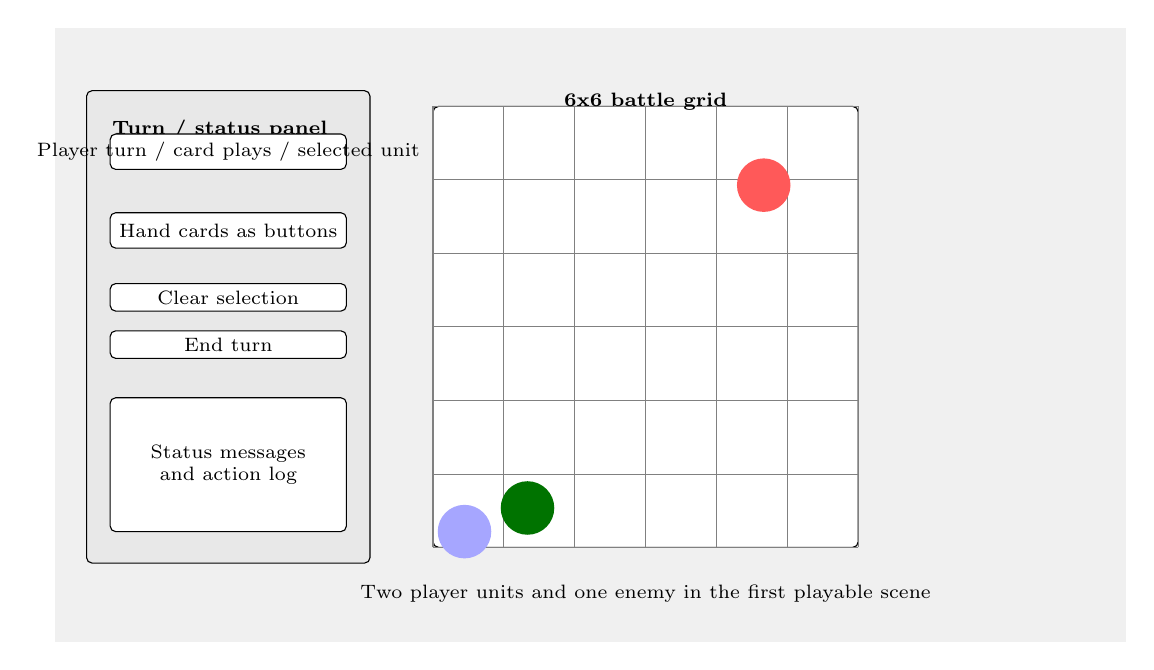
\begin{tikzpicture}[
    x=1cm,
    y=1cm,
    font=\scriptsize,
    panel/.style={draw, rounded corners=2pt, fill=gray!8},
    note/.style={draw, rounded corners=2pt, fill=white, align=center}
]
\fill[gray!12] (0,0) rectangle (13.6,7.8);

\draw[panel, fill=gray!18] (0.4,1.0) rectangle (4.0,7.0);
\node[anchor=north west] at (0.6,6.75) {\textbf{Turn / status panel}};
\draw[note] (0.7,6.0) rectangle (3.7,6.45);
\node at (2.2,6.22) {Player turn / card plays / selected unit};
\draw[note] (0.7,5.0) rectangle (3.7,5.45);
\node at (2.2,5.22) {Hand cards as buttons};
\draw[note] (0.7,4.2) rectangle (3.7,4.55);
\node at (2.2,4.37) {Clear selection};
\draw[note] (0.7,3.6) rectangle (3.7,3.95);
\node at (2.2,3.77) {End turn};
\draw[note] (0.7,1.4) rectangle (3.7,3.1);
\node[text width=2.5cm, align=center] at (2.2,2.25) {Status messages\\and action log};

\draw[panel, fill=white] (4.8,1.2) rectangle (10.2,6.8);
\foreach \x in {4.8,5.7,6.6,7.5,8.4,9.3,10.2} {
    \draw[gray] (\x,1.2) -- (\x,6.8);
}
\foreach \y in {1.2,2.13,3.07,4.0,4.93,5.87,6.8} {
    \draw[gray] (4.8,\y) -- (10.2,\y);
}
\node[anchor=north] at (7.5,7.1) {\textbf{6x6 battle grid}};
\fill[blue!35] (5.2,1.4) circle (0.34);
\fill[green!45!black] (6.0,1.7) circle (0.34);
\fill[red!65] (9.0,5.8) circle (0.34);
\node[anchor=north] at (7.5,0.85) {Two player units and one enemy in the first playable scene};
\end{tikzpicture}

\caption{Low-fidelity wireframe showing the intended information zones.}
\label{fig:retrospective-wireframe}
\end{figure}

\begin{figure}[H]
\centering

\includegraphics[width=0.88\textwidth]{battle-scene-ui.png}
\caption{Battle scene with UI, hand, and 6x6 board.}
\label{fig:prototype-evidence}
\end{figure}

\begin{figure}[H]
\centering

\includegraphics[width=0.88\textwidth]{card-hand-closeup.png}
\caption{Runtime card hand and top-bar state.}
\label{fig:prototype-cards}
\end{figure}

\begin{figure}[H]
\centering

\includegraphics[width=0.88\textwidth]{board-scene-overview.png}
\caption{Board-only view of the playable battle scene.}
\label{fig:prototype-board}
\end{figure}

The wireframe shows the intended information architecture: prompt information, a central board, and a persistent hand zone. The runtime screenshots show how that structure appears in the delivered build.

\section{Reserved Updated Screenshot Set}

The figures above preserve the earlier runtime evidence already referenced by the report. To support a clearer final comparison, the following reserved slots mark where refreshed captures from the latest build should be inserted. These newer captures are intended to sit alongside the earlier figures rather than silently replacing them.

\begin{figure}[H]
\centering
\placeholdergraphic{5.2cm}{Expected replacement: updated main-menu capture showing the branded title overlay, summary panel, and call-to-action button. Suggested file name: `title-screen-final.png`.}
\caption{Reserved slot for the updated main-menu screen, to be compared with the earlier information architecture in Figure \ref{fig:retrospective-wireframe}.}
\label{fig:updated-title-placeholder}
\end{figure}

\begin{figure}[H]
\centering
\placeholdergraphic{5.2cm}{Expected replacement: updated battle-overview capture showing the final board dressing, HUD, and unit presentation. Suggested file name: `battle-screen-final.png`.}
\caption{Reserved slot for the updated battle view, to be compared with the earlier runtime battle screenshot in Figure \ref{fig:prototype-evidence}.}
\label{fig:updated-battle-placeholder}
\end{figure}

\begin{figure}[H]
\centering
\placeholdergraphic{5.2cm}{Expected replacement: updated card-interface capture showing the hand dock, prompt bar, and action feedback. Suggested file name: `card-interface-final.png`.}
\caption{Reserved slot for the updated card-interface capture, to be compared with the earlier hand-and-top-bar view in Figure \ref{fig:prototype-cards}.}
\label{fig:updated-card-ui-placeholder}
\end{figure}

\begin{figure}[H]
\centering
\placeholdergraphic{5.2cm}{Expected replacement: representative close-up of a final card face, including icon, title, cost/action hint, and descriptive text. Suggested file name: `card-face-final.png`.}
\caption{Reserved slot for a close-up of the final card-face design.}
\label{fig:updated-card-face-placeholder}
\end{figure}

\begin{figure}[H]
\centering
\placeholdergraphic{5.2cm}{Expected replacement: victory result screen showing final end-state presentation and replay/menu actions. Suggested file name: `result-victory-final.png`.}
\caption{Reserved slot for the victory result screen, documenting the completed positive end-state flow.}
\label{fig:updated-victory-placeholder}
\end{figure}

\begin{figure}[H]
\centering
\placeholdergraphic{5.2cm}{Expected replacement: defeat result screen showing final end-state presentation and replay/menu actions. Suggested file name: `result-defeat-final.png`.}
\caption{Reserved slot for the defeat result screen, documenting the alternate end-state flow.}
\label{fig:updated-defeat-placeholder}
\end{figure}

\section{Code Structure}

The project is built around a small set of scene-bound `MonoBehaviour` scripts plus a few light model or helper types, so folder and responsibility views communicate the runtime better than a large inheritance tree would.

\begin{Verbatim}[fontsize=\small]
Assets/Scripts
|-- Cards
|   |-- CardData.cs
|   |-- CardResolver.cs
|   `-- DeckManager.cs
|-- Common
|   `-- GameEnums.cs
|-- Core
|   |-- GameFlowController.cs
|   |-- GameFlowState.cs
|   |-- GameRoot.cs
|   `-- TurnManager.cs
|-- Grid
|   |-- GridManager.cs
|   `-- TileView.cs
|-- Presentation
|   |-- UnitVisualShell.cs
|   `-- WorldThemeResources.cs
|-- UI
|   |-- BattleHudModels.cs
|   |-- BattleUI.cs
|   |-- CardButtonView.cs
|   |-- UiThemeResources.cs
|   `-- UnitHealthBarView.cs
`-- Units
    |-- EnemyAI.cs
    `-- UnitController.cs
\end{Verbatim}

The implementation stays focused on a single battle slice. The battlefield, deck flow, and enemy response remain intentionally compact so that interaction clarity and system stability take priority over content breadth.

\section{Unity Engine-Level Implementation Details}

\begin{table}[H]
\centering
\small
\begin{tabular}{lll}
\toprule
\wcell{3.2cm}{\textbf{Concern}} & \wcell{4.1cm}{\textbf{Actual implementation in the final build}} & \wcell{4.2cm}{\textbf{Reason this choice was kept}} \\
\midrule
\wcell{3.2cm}{Runtime UI root} & \wcell{4.1cm}{`GameFlowController` creates a `ScreenSpaceOverlay` `Canvas` with `CanvasScaler`, `GraphicRaycaster`, and `InputSystemUIInputModule`.} & \wcell{4.2cm}{Keeps title, battle, and result flow in one scene and simplifies testing of flow state.} \\
\wcell{3.2cm}{Board interaction path} & \wcell{4.1cm}{`BattleUI` reads `Mouse.current`, checks `EventSystem.current.IsPointerOverGameObject()`, and then uses `Physics.Raycast` for board clicks.} & \wcell{4.2cm}{Directly links card selection to tile and unit selection without building a heavier custom input layer.} \\
\wcell{3.2cm}{Tile interaction surface} & \wcell{4.1cm}{`GridManager` creates tiles as `PrimitiveType.Cube`, which provides colliders for click and occupancy interaction.} & \wcell{4.2cm}{Simple primitive generation makes the board easy to build, raycast, and validate.} \\
\wcell{3.2cm}{Presentation props} & \wcell{4.1cm}{World dressing uses generated primitives with colliders removed or disabled through the presentation helper path.} & \wcell{4.2cm}{Prevents decorative props from blocking tactical interaction while preserving scene dressing.} \\
\wcell{3.2cm}{UI-state separation} & \wcell{4.1cm}{`BattleUI` builds `BattleHudSnapshot` and card-view models instead of reading scattered fields ad hoc.} & \wcell{4.2cm}{Improves testability and reduces the risk of late HUD regressions.} \\
\wcell{3.2cm}{Debug entry path} & \wcell{4.1cm}{Direct-battle debug mode is routed through the shared flow bootstrap instead of bypassing the real HUD.} & \wcell{4.2cm}{Ensures smoke and automated checks exercise the same runtime tree the player actually sees.} \\
\bottomrule
\end{tabular}
\caption{Unity engine-level implementation details.}
\label{tab:unity-implementation-details}
\end{table}

\section{Simulation Design}

The delivered game simulates one compact tactical encounter on a 6x6 grid. Two player-controlled units occupy the board at battle start and fight one or more enemies under a turn-based loop. The simulation is deliberately deterministic: there are no random enemy tactics, no procedural map changes, and no branching objectives. This makes the battle state easier to understand for players and easier to validate for the development team.

At the start of each player turn, `TurnManager` refreshes the action budget and asks `DeckManager` to discard the previous hand and draw a new one. In the delivered build, the player draws three cards per turn and may spend two actions (`maxCardPlaysPerTurn = 2`). This keeps the turn short enough to remain readable while still allowing combinations such as move plus attack or defend plus reposition.

The fallback starter deck contains nine runtime cards:

\begin{itemize}
    \item three `Move` cards;
    \item one `Dash`;
    \item one `Strike`;
    \item one `Long Strike`;
    \item one `Guard`;
    \item one `Push`;
    \item one `Recover`.
\end{itemize}

`CardResolver` keeps the effect logic explicit. Movement and dash actions resolve against tiles, strike and push actions resolve against enemy units, and guard or recover resolve against the acting unit. Enemy behaviour remains deterministic: `EnemyAI` selects the nearest alive player unit by Manhattan distance and either attacks when adjacent or steps toward the target.

\section{UI Design}

The front-end flow is assembled at runtime by `GameFlowController`. It creates the runtime canvas, builds title, battle, and result panels, and keeps them inside the same main scene. The title panel includes the game brand, a short summary, a feature strip, and a clear call to action. The result panel exposes the battle outcome plus replay and menu actions.

During battle, `BattleUI` builds a three-zone runtime HUD:

\begin{itemize}
    \item a top bar for turn state, remaining energy, selection state, prompts, and action buttons;
    \item a left panel for unit summary, status, and the battle log;
    \item a bottom panel for the active hand of cards.
\end{itemize}

The runtime HUD does not pull ad hoc strings directly from scattered private state. Instead, it builds a `BattleHudSnapshot` containing turn labels, prompt text, selected-unit information, card states, and unit summaries. `CardButtonView` uses this snapshot to render card title, description, use hints, and disabled reasons directly in the hand. `UnitHealthBarView` projects health state back into world space so HP can be read from the board rather than only from the log.

Visual theming is added without replacing the project's own runtime structure. The interface uses themed UI resources for banners, panels, buttons, and symbols, while the board, props, and unit silhouettes remain driven by the project's own presentation code. The result is still a compact demo, but it now looks intentional rather than merely assembled.

\chapter{Test \& System Evaluation}

Testing became the main backbone of the project during WR3 and remained central during the post-WR3 completion push. The final validation approach did not rely on a single type of evidence. Instead, it combined direct EditMode tests for stable logic, PlayMode smoke for whole-scene readiness, and manual smoke for visual composition and overlay-heavy UI behaviour \cite{cw1Specification,wr3ExecutionSummary,postWr3IssueLog}.

\section{Test Strategy}

The core strategy was \textit{TDD-first where behaviour is deterministic, smoke-first where the result is primarily visual}. This mattered because \projectname{} contains both rule-driven systems and presentation-heavy systems. Turn flow, deck lifecycle, movement constraints, damage handling, and battle-end state all have explicit success conditions and can be tested directly. By contrast, title-panel readability, overlay composition, and the visual relationship between the board and the hand dock cannot be reduced safely to screenshot-perfect automation in the current project setup.

The team therefore treated a result as \textit{verified} only when it was backed by an explicit rerun record on disk. In practice this meant that a test file, smoke note, or issue closure was not treated as complete merely because the code existed. It had to be rerun or re-smoked after the relevant fix. This rule was inherited from WR3 and remained useful during the later UI and UX passes.

Table \ref{tab:validation-layers} summarises the final validation layers.

\begin{table}[H]
\centering
\small
\begin{tabular}{llll}
\toprule
\wcell{2.2cm}{\textbf{Layer}} & \wcell{3.4cm}{\textbf{Main purpose}} & \wcell{4.3cm}{\textbf{Representative evidence}} & \wcell{2.0cm}{\textbf{Used for}} \\
\midrule
\wcell{2.2cm}{EditMode tests} & \wcell{3.4cm}{Directly verify deterministic rules and state transitions} & \wcell{4.3cm}{`TurnManagerTests`, `DeckManagerTests`, `CardResolverTests`, `GridManagerTests`, `GameFlowControllerTests`, `BattleUITests`} & \wcell{2.0cm}{Core logic, flow, UI regressions} \\
\wcell{2.2cm}{PlayMode smoke} & \wcell{3.4cm}{Verify that the scene reaches a playable runtime state} & \wcell{4.3cm}{`BattleFlowPlayModeTests`} & \wcell{2.0cm}{Scene bootstrap and battle readiness} \\
\wcell{2.2cm}{Manual smoke} & \wcell{3.4cm}{Confirm readability, layout, and aesthetic stability} & \wcell{4.3cm}{Post-WR3 UX, ambience, and HUD smoke records} & \wcell{2.0cm}{Overlay composition and final UX judgement} \\
\bottomrule
\end{tabular}
\caption{Validation layers used by the final project.}
\label{tab:validation-layers}
\end{table}

\section{Test Methods}

The automated suite is organised by runtime responsibility. This mirrors the source-tree structure and makes failures easier to interpret. The earlier WR3 validation freeze already covered the main prototype classes directly. Post-WR3 work then expanded that base by adding stronger UI and flow tests, including `GameFlowControllerTests` and additional `BattleUITests` around runtime HUD layout, disabled-card states, and direct-battle start behaviour.

At the latest post-WR3 HUD feedback checkpoint, the project reported:

\begin{itemize}
    \item `81/81` passing EditMode tests;
    \item `1/1` passing PlayMode smoke test.
\end{itemize}

This is materially stronger than the WR3 freeze alone because the later counts include the new title-flow, HUD, and layout-regression work. Table \ref{tab:final-execution-summary} shows the progression from the archived WR3 validation baseline into the later post-WR3 reruns.

\begin{table}[H]
\centering
\small
\begin{tabular}{lllll}
\toprule
\wcell{2.0cm}{\textbf{Checkpoint}} & \wcell{2.1cm}{\textbf{EditMode}} & \wcell{2.0cm}{\textbf{PlayMode}} & \wcell{3.3cm}{\textbf{Primary focus}} & \wcell{2.4cm}{\textbf{Evidence source}} \\
\midrule
\wcell{2.0cm}{WR3 freeze\\(17/04/2026)} & \wcell{2.1cm}{`57/57`} & \wcell{2.0cm}{`1/1`} & \wcell{3.3cm}{Battle-loop validation and requirements coverage freeze} & \wcell{2.4cm}{WR3 execution summary} \\
\wcell{2.0cm}{M12 ambience\\(24/04/2026)} & \wcell{2.1cm}{`75/75`} & \wcell{2.0cm}{`1/1`} & \wcell{3.3cm}{World-layer presentation pass and title/result dressing} & \wcell{2.4cm}{Ambience smoke record} \\
\wcell{2.0cm}{M13 HUD feedback\\(24/04/2026)} & \wcell{2.1cm}{`81/81`} & \wcell{2.0cm}{`1/1`} & \wcell{3.3cm}{HUD readability, disabled-card feedback, and layout regression closure} & \wcell{2.4cm}{HUD feedback smoke record} \\
\bottomrule
\end{tabular}
\caption{Progression from the WR3 validation baseline to the final post-WR3 reruns.}
\label{tab:final-execution-summary}
\end{table}

The suite now covers the main runtime concerns directly:

\begin{itemize}
    \item battle start, battle end, and turn-loop correctness;
    \item draw, discard, reshuffle, and hand lifecycle;
    \item movement, attack, push, guard, heal, and occupancy rules;
    \item enemy target selection and movement decisions;
    \item battle HUD prompts, disabled-card reasoning, and runtime layout guards;
    \item title-flow and result-flow state transitions.
\end{itemize}

This is important because the final project was not only judged on whether the game happened to run during a demo. It was also judged on whether the team could show systematic validation around the delivered behaviour.

\section{Code Coverage}

The project does have an archived code-coverage baseline from the WR3 validation freeze. That archive recorded:

\begin{itemize}
    \item `11` runtime classes in the coverage report;
    \item `74.2\%` line coverage;
    \item `92.4\%` method coverage.
\end{itemize}

Those figures come from the 17/04/2026 archived coverage export and are useful because they quantify the validation position at the point where the prototype battle slice was formally frozen for WR3 \cite{wr3ExecutionSummary}. They also show that the suite was not limited to a few smoke assertions; it already covered most of the core runtime surface directly.

However, the report must stay honest about the current limitation: the coverage archive has not yet been regenerated after the post-WR3 expansion from the WR3 baseline to the later `81/81` EditMode position. In addition, the current worktree shows the archived coverage folder in a dirty state. For that reason, the final report should treat the `74.2\%` line-coverage figure as an archived WR3 baseline rather than claim it as the final post-polish coverage number. The correct next step before final submission is to restore or regenerate the archive and then update the chapter if a final-coursework coverage figure is required.

This distinction matters because coverage is only useful when tied to a known suite state. Reporting a stale number as if it belongs to the latest build would weaken the credibility of the report.

\section{Evaluation}

The delivered build satisfies the main goal of the project: it provides a complete and readable tactical battle loop rather than only a technical prototype. The player can begin from a title screen, enter battle, select units and cards, understand the turn state through the HUD, observe enemy response, and reach a result screen with replay or menu options. The core gameplay, runtime flow, and late-stage usability improvements are all supported by named evidence on disk.

Table \ref{tab:final-evaluation-summary} summarises the main outcome areas.

\begin{table}[H]
\centering
\small
\begin{tabular}{lll}
\toprule
\wcell{3.8cm}{\textbf{Area}} & \wcell{2.0cm}{\textbf{Outcome}} & \wcell{5.4cm}{\textbf{Reasoning}} \\
\midrule
\wcell{3.8cm}{Playable front-end flow} & \wcell{2.0cm}{Satisfied} & \wcell{5.4cm}{Title, battle, and result states now exist inside the main scene and are covered by flow and smoke evidence.} \\
\wcell{3.8cm}{Battle rules and turn loop} & \wcell{2.0cm}{Satisfied} & \wcell{5.4cm}{Movement, attack, guard, push, recover, draw/discard, enemy turns, and battle-end handling are directly tested.} \\
\wcell{3.8cm}{HUD readability and action feedback} & \wcell{2.0cm}{Satisfied} & \wcell{5.4cm}{Energy, prompts, disabled-card reasons, and world-space health bars closed earlier readability gaps.} \\
\wcell{3.8cm}{Visual and thematic cohesion} & \wcell{2.0cm}{Satisfied} & \wcell{5.4cm}{Themed UI assets, board ambience, and silhouette-based units now give the slice a coherent visual direction.} \\
\wcell{3.8cm}{Regression protection} & \wcell{2.0cm}{Satisfied} & \wcell{5.4cm}{Late-stage UI and flow fixes were backed by reruns, not only by one-off manual checks.} \\
\wcell{3.8cm}{Residual limitations} & \wcell{2.0cm}{Open but non-blocking} & \wcell{5.4cm}{The project remains a single-battle demo, overlay-heavy screenshot capture still needs manual smoke, and coverage needs a fresh post-polish export.} \\
\bottomrule
\end{tabular}
\caption{Final evaluation summary for the delivered build.}
\label{tab:final-evaluation-summary}
\end{table}

The most valuable aspect of the final testing cycle is not any single number. It is the fact that the major late-stage defects were turned into explicit closure work. Title overlay collision, top-bar overlap, hand-panel occlusion, hidden card-availability feedback, and debug-flow bypass were all identified through smoke, traced to specific runtime causes, fixed in code, and then backed by rerun or hierarchy evidence. This is exactly the kind of test-and-improve loop the coursework expects \cite{postWr3IssueLog}.

The final system still has clear boundaries. It is not a large tactics game; it is a polished single-battle coursework slice. That is acceptable because the evaluation criteria reward rigour, traceability, and professionalism more than raw feature count. On that basis, the delivered build is much stronger than the early prototype: it is now a complete, demonstrable, and substantially validated software artifact rather than only a promising design idea.

\chapter{Extensibility \& Maintenance}

Although \projectname{} is a compact prototype, the delivered system is structured so that it can be maintained and extended without structural rework.

\section{Delivered Maintainability Measures}

The codebase is structured around functional responsibility rather than scene-specific scripts. Core bootstrap and flow classes are separated from battle rules, card resolution, unit logic, grid state, UI presentation, and purely visual wrappers. This makes it possible to modify one layer without rewriting the others. For example, the title flow, HUD layout, disabled-card messaging, and health-bar presentation can change without replacing the underlying turn model or card resolver.

Assembly definitions provide a second maintainability guardrail. Runtime code is grouped in the main `TacticalCards` assembly, while EditMode and PlayMode test suites are isolated in separate test assemblies. This separation reduces build pollution, avoids test-only dependencies leaking into player-facing code, and makes the validation boundary easier to explain.

Third-party assets are also contained deliberately. Imported interface art is kept separate from the battle rules and runtime state logic. This means the visual theme can be updated or replaced without having to disentangle it from gameplay behaviour.

\section{Deferred Work and Future Evolution}

The most important deferred work is content expansion, not systems rescue. The delivered game does not include a campaign structure, multiple maps, progression systems, deep deck customisation, or a large enemy catalogue. Those omissions are intentional because each of them would multiply test surface, UI complexity, and content production cost without improving the quality of the core tactical slice.

\begin{table}[H]
\centering
\small
\begin{tabular}{llll}
\toprule
\wcell{3.2cm}{\textbf{Follow-up direction}} & \wcell{4.0cm}{\textbf{What would be added}} & \wcell{2.1cm}{\textbf{Rough effort}} & \wcell{2.2cm}{\textbf{Why it was deferred}} \\
\midrule
\wcell{3.2cm}{Encounter variety} & \wcell{4.0cm}{More objectives, alternate spawn patterns, and one or two additional maps.} & \wcell{2.1cm}{1--2 weeks} & \wcell{2.2cm}{Would widen the test surface and increase tuning cost.} \\
\wcell{3.2cm}{Character presentation} & \wcell{4.0cm}{Replace procedural silhouettes with coherent character assets and simple animation.} & \wcell{2.1cm}{1 week} & \wcell{2.2cm}{HUD readability and battle clarity had higher priority.} \\
\wcell{3.2cm}{Coverage refresh} & \wcell{4.0cm}{Regenerate the coverage archive after the latest UI and flow additions.} & \wcell{2.1cm}{1--2 days} & \wcell{2.2cm}{The existing archive is still the last stable quantitative baseline.} \\
\wcell{3.2cm}{Broader PlayMode journeys} & \wcell{4.0cm}{Add more end-to-end PlayMode paths for win, loss, replay, and menu return.} & \wcell{2.1cm}{2--3 days} & \wcell{2.2cm}{EditMode coverage and targeted smoke had more immediate value.} \\
\bottomrule
\end{tabular}
\caption{Concrete extension paths with rough effort estimates.}
\label{tab:future-work-estimates}
\end{table}

The current architecture already shows that the project can absorb flow, HUD, and theming extensions in thin slices without destabilising the entire battle loop.

\chapter{Problem \& Reflections}

Many of the hardest problems in this project were not purely visual and not purely logical. In practice, presentation, interaction, testing, and planning were tightly coupled. Once the interface became more elaborate, every UI change exposed another layer of engineering work: raycast boundaries, runtime layout assumptions, battle-state messaging, or proof that a fix had actually held. This chapter reflects on those issues at technical, project-management, and team-management levels.

\section{Technical Problem}

One recurring technical problem was that visual polish changed interaction behaviour. As the title overlay, themed HUD, and hand dock became more elaborate, previously hidden assumptions in the prototype started to fail. Concrete examples included title overlay content colliding vertically, the top-left prompt stack overlapping turn and energy labels, the hand dock obscuring lower units, and action availability being visible only in the battle log.

The important lesson was that these defects could not be handled with visual tweaking alone. Several bugs existed at the boundary between layout and logic. A panel could look harmless but still intercept clicks; a debug shortcut could speed up testing but bypass the same flow path used by the real HUD; a screenshot could show the board correctly while missing overlay elements entirely.

Another technical limitation came from tooling. Overlay screenshots were not always trustworthy for `Screen Space Overlay` verification in this setup. The practical response was to split validation responsibility: hierarchy assertions and runtime tests for structural proof, and manual smoke for final overlay readability.

\section{Project Management}

From a project-management perspective, the main challenge was resisting attractive but expensive scope growth. The game concept could easily have drifted toward a larger tactics RPG with more cards, more maps, more animation, and progression systems. Instead, the team kept returning to the vertical-slice rule: build one encounter well, then extend only when the current layer is stable.

This project-management choice is closely related to the development model described in Chapter 4. The team worked iteratively in a lightweight agile style, regularly returning to the backlog after each usable slice \cite{agileManifesto2001}. That proved more appropriate than trying to freeze all design decisions up front in a strict sequential process, especially once visible usability problems began to emerge. In retrospect, this also matches Royce's warning that large software work becomes risky when treated as a simple one-pass flow \cite{royce1970}.

Testing and evidence collection also became planning tools rather than only reporting tasks. When a feature area lacked a clear validation path, that was treated as a planning warning sign. Improvements such as disabled-card overlays, world-space health bars, and menu-flow fixes were prioritised because they closed real usability gaps and could be backed by tests or smoke evidence. Cosmetic work that could not yet be validated or stabilised was deprioritised.

\section{Team Management}

The team-management story is more mixed, and it is important to describe it honestly. Early coordination relied more on informal communication and shared files than on a fully preserved repository-first workflow. Later, the project converged onto a clearer branch-and-merge model with a stronger evidence tree. That change improved accountability and made the final codebase and report trail easier to audit, but it also meant that some early process context had to be preserved as recovered notes rather than as perfect historical records.

This was not only an administrative issue. It affected how the team divided work and reviewed risk. Once responsibilities, issue logs, screenshots, and report material lived in the same workspace, ambiguity reduced sharply. Code ownership became easier to follow, design changes became easier to justify, and late-stage fixes became easier to validate collaboratively.

The most positive team-management lesson is therefore standardisation. The project became stronger once the team treated one repository, one evidence tree, and one final-report source as the canonical workspace. The most important remaining weakness is that this standardisation happened later than ideal, so the report must still be transparent about which early records are formal and which are recovered.

\chapter{Conclusion}

This project delivered a complete and submission-ready tactical card battle prototype in Unity. The final build provides a coherent front-end flow, a functioning card-driven skirmish on a grid, readable battle feedback, a result state, documented open-asset use, and a validation trail that extends from requirements through tests, smoke checks, and issue closure. The system remains intentionally small, but that small scope is one of its strengths: it allowed the team to finish a real vertical slice rather than leave a larger design half-implemented.

The final report also shows that the most valuable work was not only in adding features, but in making the prototype explainable and maintainable. Post-WR3 milestones improved the title flow, battle HUD, usability feedback, and visual presentation while preserving the core turn model and strengthening the test package. Remaining limitations are mainly additive: more encounter variety, richer characters and animation, and a refreshed final-stage coverage snapshot would all improve the project, but none of them are required to understand or play the delivered game.

Overall, \projectname{} meets the coursework goal of combining a game product with defensible software-engineering practice. It demonstrates a compact but complete tactical design, a stable implementation path, and a documented process that is strong enough to support final submission and future extension.


\newpage
\addcontentsline{toc}{chapter}{Reference}
\bibliographystyle{plain}
\bibliography{references}

\appendix

\chapter{User Manual}
\section{Purpose}

This manual explains how to run and play the current \projectname{} demo in the Unity Editor. The delivered coursework build is a compact single-battle prototype rather than a full campaign game, so the manual focuses on the playable battle loop and the runtime HUD.

\section{Opening the Project}

\begin{enumerate}
    \item Open the Unity project located in \code{coursework/}.
    \item Load \code{Assets/Scenes/SampleScene.unity}.
    \item Press the Unity Editor \texttt{Play} button.
\end{enumerate}

When the scene starts correctly, the player first sees the title screen rather than entering combat immediately.

\section{Starting a Battle}

\begin{enumerate}
    \item Wait for the title screen to finish loading.
    \item Press \texttt{Start Battle}.
    \item The game transitions into the battle state and the battle HUD becomes active.
\end{enumerate}

If the battle has already finished, the result screen allows the player to replay the battle or return to the title screen.

\section{Core Interaction Flow}

The intended interaction order during the player turn is:

\begin{enumerate}
    \item select a player unit on the board;
    \item select a card from the hand;
    \item select a valid target tile or enemy unit if the card requires one;
    \item observe the result and continue until the turn ends.
\end{enumerate}

The player can press \texttt{Clear} to reset the current selection and \texttt{End Turn} to pass control to the enemy phase.

\section{Reading the Battle HUD}

\subsection{Top Bar}

The top bar provides the most important turn-state information:

\begin{itemize}
    \item current turn state;
    \item remaining action budget, shown as \texttt{Energy};
    \item current selection state;
    \item prompt text describing what the player should do next.
\end{itemize}

\subsection{Left Panel}

The left panel provides supporting battle information:

\begin{itemize}
    \item unit summary;
    \item battle log;
    \item recent action history.
\end{itemize}

\subsection{Bottom Hand Panel}

The bottom panel displays the current hand of cards. Each card includes:

\begin{itemize}
    \item card name;
    \item action type;
    \item effect summary such as range, damage, movement, or recovery value.
\end{itemize}

When a card cannot be used in the current state, the card shows disabled feedback directly instead of relying only on the battle log.

\subsection{World-space Unit Feedback}

Each unit displays a world-space health bar above the model. This allows the player to read board state without scanning the text log after every action.

\section{Card Reference}

The current fallback starter deck supports the following actions:

\begin{itemize}
    \item \textbf{Move}: move the selected unit up to 2 tiles.
    \item \textbf{Dash}: move the selected unit up to 3 tiles.
    \item \textbf{Strike}: deal 2 damage to an adjacent enemy.
    \item \textbf{Long Strike}: deal 2 damage to an enemy within 2 tiles.
    \item \textbf{Guard}: reduce the next incoming hit against the selected unit.
    \item \textbf{Push}: deal 1 damage and push the enemy backward if possible.
    \item \textbf{Recover}: restore 2 health to the selected unit.
\end{itemize}

\section{Understanding the Turn Loop}

\begin{enumerate}
    \item At the start of the player turn, the game refreshes the action budget and hand state.
    \item The player performs a limited number of card-driven actions.
    \item The player ends the turn.
    \item Enemy units execute their actions automatically.
    \item The game checks whether the battle should continue or end in victory or defeat.
\end{enumerate}

Some battles may introduce reinforcement pressure during play. This is an intended part of the final tactical slice.

\section{Ending the Battle}

When the battle reaches a win or loss condition, the runtime flow changes to the result screen. The result screen provides:

\begin{itemize}
    \item a visible battle outcome;
    \item replay/start-over behaviour;
    \item a return path to the title screen.
\end{itemize}

\section{Troubleshooting}

\begin{itemize}
    \item If the title screen does not appear, verify that \code{SampleScene.unity} is the loaded scene and that the project compiled successfully.
    \item If a card cannot be played, check the current prompt text, selection state, and the card's disabled feedback.
    \item If board state becomes hard to follow, use the top-bar prompt plus the world-space health bars before relying on the battle log.
\end{itemize}


\chapter{Meeting Minutes}
\section{Evidence Status}

This appendix preserves the meeting evidence currently archived in the workspace. One early checkpoint is reconstructed from dated project artifacts rather than preserved as a full formal minute set, so it remains explicitly labelled as \textit{recovered}. That distinction is kept visible instead of being hidden.

\begin{table}[H]
\centering
\small
\begin{tabular}{llll}
\toprule
\wcell{3.0cm}{\textbf{Record}} & \wcell{1.9cm}{\textbf{Date}} & \wcell{2.5cm}{\textbf{Type}} & \wcell{4.2cm}{\textbf{Current use}} \\
\midrule
\wcell{3.0cm}{Recovered early implementation checkpoint} & \wcell{1.9cm}{15/03/2026} & \wcell{2.5cm}{Recovered note} & \wcell{4.2cm}{Explains the first playable scope and early implementation decisions.} \\
\wcell{3.0cm}{Kickoff meeting} & \wcell{1.9cm}{17/03/2026} & \wcell{2.5cm}{Formal note} & \wcell{4.2cm}{Shows initial direction-setting and role alignment.} \\
\wcell{3.0cm}{Scope alignment meeting} & \wcell{1.9cm}{18/03/2026} & \wcell{2.5cm}{Formal note} & \wcell{4.2cm}{Shows agreement on tactical-battle scope and documentation format.} \\
\wcell{3.0cm}{Validation planning meeting} & \wcell{1.9cm}{15/04/2026} & \wcell{2.5cm}{Formal note} & \wcell{4.2cm}{Shows testing strategy, defect triage, and final validation planning.} \\
\bottomrule
\end{tabular}
\caption{Meeting evidence preserved in the final-report appendix.}
\label{tab:appendix-meeting-register}
\end{table}

\section{Recovered Early Implementation Checkpoint}

\textbf{Date:} 15/03/2026 \\
\textbf{Type:} recovered from local implementation artifacts \\
\textbf{Attendance:} exact attendance not preserved in the workspace

\subsection{Purpose}

Define the minimum playable slice that could demonstrate the project idea in software rather than only in prose.

\subsection{Recovered Decisions}

\begin{itemize}
    \item Keep one battle scene for the first playable version.
    \item Fix the board at 6x6 so movement, targeting, and occupancy remain readable.
    \item Limit the first playable card set to Move, Strike, Guard, and Push.
    \item Use one shared `UnitController` for player and enemy units.
    \item Keep enemy behaviour deterministic.
    \item Use button-based card selection instead of drag-and-drop.
\end{itemize}

\subsection{Recovered Follow-up}

\begin{itemize}
    \item Implement the first-pass script set and scene bootstrap.
    \item Refresh diagrams so they match the code actually built.
    \item Capture early prototype screenshots.
    \item Start separating validation notes from design notes.
\end{itemize}

\section{Kickoff Meeting}

\textbf{Date:} 17/03/2026 \\
\textbf{Attendance:} Guangjun HU, Hongshuo HU, Zehan CHEN

\subsection{Context}

The team compared initial game ideas, narrowed the project direction, and assigned the first requirement and planning tasks.

\subsection{Decisions}

\begin{itemize}
    \item Confirm \projectname{} as the chosen project direction.
    \item Agree initial role allocation.
    \item Set the first delivery expectations for requirements and design material.
\end{itemize}

\section{Scope Alignment Meeting}

\textbf{Date:} 18/03/2026 \\
\textbf{Attendance:} Guangjun HU, Cheng YE

\subsection{Context}

This meeting aligned the project around a tactical card battle demo and standardised a lightweight documentation format for later work.

\subsection{Decisions}

\begin{itemize}
    \item Keep the software scope focused on a tactical card battle rather than a larger campaign game.
    \item Assign UML and design-diagram production.
    \item Use a repeatable meeting-note structure for later checkpoints.
\end{itemize}

\section{Validation Planning Meeting}

\textbf{Date:} 15/04/2026 \\
\textbf{Format:} Online \\
\textbf{Chair:} Guangjun HU \\
\textbf{Secretary:} Zehan CHEN

\subsection{Attendance}

\begin{itemize}
    \item Guangjun HU -- present
    \item Hongshuo HU -- present
    \item Cheng YE -- present
    \item Zehan CHEN -- present
\end{itemize}

\subsection{Agenda}

\begin{enumerate}
    \item Review usability findings from the playable build.
    \item Confirm automated-test scope and smoke responsibilities.
    \item Allocate drafting tasks for the final validation material.
    \item Set deadlines for open defects and reruns.
\end{enumerate}

\subsection{Key Decisions}

\begin{itemize}
    \item Treat deterministic behaviour as regression-test candidates and keep manual smoke for overlay-heavy UI concerns.
    \item Require rerun-backed evidence before a visible issue can be considered closed.
    \item Keep late work focused on flow, HUD, and readability rather than widening the feature set.
\end{itemize}

\subsection{Action Items}

\begin{table}[H]
\centering
\footnotesize
\setlength{\tabcolsep}{4pt}
\begin{tabular}{llll}
\toprule
\wcell{4.1cm}{\textbf{Task}} & \wcell{2.0cm}{\textbf{Owner}} & \wcell{1.8cm}{\textbf{Due}} & \wcell{2.8cm}{\textbf{Review owner}} \\
\midrule
\wcell{4.1cm}{Draft report sections and supporting tables} & \wcell{2.0cm}{Cheng YE} & \wcell{1.8cm}{16/04/2026} & \wcell{2.8cm}{Guangjun HU} \\
\wcell{4.1cm}{Run EditMode tests and archive results} & \wcell{2.0cm}{Hongshuo HU} & \wcell{1.8cm}{15/04/2026} & \wcell{2.8cm}{Guangjun HU} \\
\wcell{4.1cm}{Update defect register and meeting notes} & \wcell{2.0cm}{Zehan CHEN} & \wcell{1.8cm}{16/04/2026} & \wcell{2.8cm}{Cheng YE} \\
\wcell{4.1cm}{Run final integration check in Unity} & \wcell{2.0cm}{Hongshuo HU} & \wcell{1.8cm}{17/04/2026} & \wcell{2.8cm}{Whole team} \\
\bottomrule
\end{tabular}
\caption{Action items from the validation planning meeting.}
\label{tab:appendix-validation-actions}
\end{table}


\chapter{Test Case}
\section{Validation Evidence Register}

\begin{table}[H]
\centering
\small
\begin{tabular}{llll}
\toprule
\wcell{3.2cm}{\textbf{Evidence item}} & \wcell{1.8cm}{\textbf{Date}} & \wcell{2.2cm}{\textbf{Type}} & \wcell{4.3cm}{\textbf{Use in the report}} \\
\midrule
\wcell{3.2cm}{Prototype accuracy regression run} & \wcell{1.8cm}{02/04/2026} & \wcell{2.2cm}{EditMode run} & \wcell{4.3cm}{Shows the battle-end correctness fix was rerun and closed.} \\
\wcell{3.2cm}{Archived validation summary} & \wcell{1.8cm}{17/04/2026} & \wcell{2.2cm}{Execution record} & \wcell{4.3cm}{Provides the archived baseline suite counts and coverage export.} \\
\wcell{3.2cm}{Coverage export snapshot} & \wcell{1.8cm}{17/04/2026} & \wcell{2.2cm}{Coverage record} & \wcell{4.3cm}{Provides the quantitative line and method coverage baseline.} \\
\wcell{3.2cm}{Defect and retest register} & \wcell{1.8cm}{17/04/2026} & \wcell{2.2cm}{Defect log} & \wcell{4.3cm}{Shows which inherited or current defects were closed through rerun evidence.} \\
\wcell{3.2cm}{Visual ambience smoke} & \wcell{1.8cm}{24/04/2026} & \wcell{2.2cm}{Manual smoke} & \wcell{4.3cm}{Shows the themed board and scene dressing stayed stable.} \\
\wcell{3.2cm}{HUD feedback smoke} & \wcell{1.8cm}{24/04/2026} & \wcell{2.2cm}{Manual smoke} & \wcell{4.3cm}{Shows the final HUD layout and interaction feedback remained readable.} \\
\wcell{3.2cm}{Late-stage UI and HUD issue log} & \wcell{1.8cm}{24/04/2026} & \wcell{2.2cm}{Issue log} & \wcell{4.3cm}{Explains how the final visual defects were found and closed.} \\
\bottomrule
\end{tabular}
\caption{Main validation records preserved for the final report.}
\label{tab:appendix-validation-register}
\end{table}

\section{Coverage Snapshot}

The appendix preserves two complementary views of validation:

\begin{itemize}
    \item an archived quantitative coverage snapshot;
    \item later rerun counts after the final flow and HUD passes.
\end{itemize}

\begin{table}[H]
\centering
\small
\begin{tabular}{lll}
\toprule
\wcell{3.4cm}{\textbf{Metric}} & \wcell{2.4cm}{\textbf{Value}} & \wcell{4.9cm}{\textbf{Interpretation}} \\
\midrule
\wcell{3.4cm}{Archived runtime classes} & \wcell{2.4cm}{`11`} & \wcell{4.9cm}{The archived coverage report covers the core runtime slice.} \\
\wcell{3.4cm}{Archived line coverage} & \wcell{2.4cm}{`74.2\%`} & \wcell{4.9cm}{Useful quantitative baseline before the final polishing passes.} \\
\wcell{3.4cm}{Archived method coverage} & \wcell{2.4cm}{`92.4\%`} & \wcell{4.9cm}{Shows strong method-level closure for the deterministic battle systems.} \\
\wcell{3.4cm}{Latest EditMode rerun} & \wcell{2.4cm}{`81/81`} & \wcell{4.9cm}{Shows the suite expanded after later flow and HUD work.} \\
\wcell{3.4cm}{Latest PlayMode rerun} & \wcell{2.4cm}{`1/1`} & \wcell{4.9cm}{Shows the playable scene still boots and reaches battle readiness.} \\
\bottomrule
\end{tabular}
\caption{Coverage and rerun snapshot preserved in the appendix.}
\label{tab:appendix-coverage-snapshot}
\end{table}

\section{Representative Automated Test Inventory}

\begin{table}[H]
\centering
\small
\begin{tabular}{lll}
\toprule
\wcell{2.8cm}{\textbf{Area}} & \wcell{4.7cm}{\textbf{Representative suites}} & \wcell{4.0cm}{\textbf{What they protect}} \\
\midrule
\wcell{2.8cm}{Battle bootstrap} & \wcell{4.7cm}{`GameRootTests`, `GameFlowControllerTests`} & \wcell{4.0cm}{Flow transitions, runtime UI creation, replay/menu behaviour} \\
\wcell{2.8cm}{Turn loop} & \wcell{4.7cm}{`TurnManagerTests`} & \wcell{4.0cm}{Action budget, battle-end rules, enemy-phase handoff} \\
\wcell{2.8cm}{Cards and deck} & \wcell{4.7cm}{`DeckManagerTests`, `CardResolverTests`} & \wcell{4.0cm}{Draw/discard lifecycle and card-effect branches} \\
\wcell{2.8cm}{Grid and tiles} & \wcell{4.7cm}{`GridManagerTests`, `TileViewTests`} & \wcell{4.0cm}{Placement, occupancy, range, and highlight behaviour} \\
\wcell{2.8cm}{Units and AI} & \wcell{4.7cm}{`UnitControllerTests`, `EnemyAITests`} & \wcell{4.0cm}{Damage, healing, guard, target choice, and movement} \\
\wcell{2.8cm}{HUD and card views} & \wcell{4.7cm}{`BattleUITests`, `CardButtonViewTests`} & \wcell{4.0cm}{Prompt layout, disabled-card states, and layout regression guards} \\
\wcell{2.8cm}{Playable-scene readiness} & \wcell{4.7cm}{`BattleFlowPlayModeTests`} & \wcell{4.0cm}{Scene bootstrap and battle entry in Play Mode} \\
\bottomrule
\end{tabular}
\caption{Representative automated test coverage in the delivered project.}
\label{tab:appendix-test-inventory}
\end{table}

\section{Manual Smoke Checklist}

The following player-visible checks were retained as manual smoke responsibilities:

\begin{itemize}
    \item title screen loads and the start button is readable;
    \item battle HUD appears without text overlap;
    \item opening hand dock does not obscure the lower board excessively;
    \item victory and defeat both reach the result state cleanly;
    \item disabled cards explain why they cannot be played;
    \item world-space health bars remain readable during combat.
\end{itemize}


\chapter{Development Planning}
\section{Iterative Delivery Model}

The project was delivered in short increments rather than as a once-through sequential build. The repository history shows repeated cycles of implementation, playable checking, design revision, validation, and interface refinement.

\begin{table}[H]
\centering
\small
\begin{tabular}{llll}
\toprule
\wcell{2.6cm}{\textbf{Iteration window}} & \wcell{3.6cm}{\textbf{Representative commits}} & \wcell{3.6cm}{\textbf{Primary focus}} & \wcell{2.6cm}{\textbf{Outcome}} \\
\midrule
\wcell{2.6cm}{01/04--02/04} & \wcell{3.6cm}{\code{22b36f4}, \code{b045777}, \code{814c972}, \code{f2ac529}} & \wcell{3.6cm}{Repository curation, clean baseline, battle-end correction, initial regression protection} & \wcell{2.6cm}{A stable prototype baseline with an early correctness fix} \\
\wcell{2.6cm}{02/04--03/04} & \wcell{3.6cm}{\code{968d396}, \code{7438df9}, \code{2d6a444}, \code{e407e63}} & \wcell{3.6cm}{Architecture alignment, screenshots, diagrams, and code/report consistency} & \wcell{2.6cm}{A reportable prototype with aligned visual and structural evidence} \\
\wcell{2.6cm}{17/04} & \wcell{3.6cm}{\code{c78434f}} & \wcell{3.6cm}{Validation freeze and archived rerun evidence} & \wcell{2.6cm}{A named baseline for execution and coverage evidence} \\
\wcell{2.6cm}{23/04} & \wcell{3.6cm}{\code{b8c1ab3}} & \wcell{3.6cm}{Title-to-result flow shell, gameplay stability, and stronger test coverage} & \wcell{2.6cm}{A complete session loop rather than battle-only entry} \\
\wcell{2.6cm}{23/04--24/04} & \wcell{3.6cm}{\code{c4fa026}, \code{572acb2}} & \wcell{3.6cm}{Runtime UI theming, board dressing, and unit presentation} & \wcell{2.6cm}{A stronger visual identity without changing the core rules} \\
\wcell{2.6cm}{24/04} & \wcell{3.6cm}{\code{98753ae}} & \wcell{3.6cm}{HUD feedback closure, overlay repair, and layout fixes} & \wcell{2.6cm}{The last major usability gaps were closed} \\
\wcell{2.6cm}{24/04} & \wcell{3.6cm}{\code{df9ea5a}} & \wcell{3.6cm}{Final report package preparation} & \wcell{2.6cm}{The report source tree and final-document scaffolding were assembled} \\
\bottomrule
\end{tabular}
\caption{Representative iterative slices visible in the repository history.}
\label{tab:appendix-iteration-history}
\end{table}

\section{Backlog Reprioritisation Logic}

The team did not treat the plan as fixed after the first playable build. The backlog was reprioritised when direct evidence showed a more urgent need. In practice, the reprioritisation rule was:

\begin{enumerate}
    \item keep the core tactical slice playable at all times;
    \item promote any defect that blocks understanding, battle completion, or report credibility;
    \item defer attractive but expensive content work if it does not improve the current slice materially.
\end{enumerate}

This logic is why session flow, HUD readability, and regression protection were prioritised above wider content expansion.


\chapter{Version Control}
\section{Workflow Summary}

\begin{table}[H]
\centering
\small
\begin{tabular}{lll}
\toprule
\wcell{3.2cm}{\textbf{Practice}} & \wcell{4.3cm}{\textbf{How it was applied}} & \wcell{4.1cm}{\textbf{Why it mattered}} \\
\midrule
\wcell{3.2cm}{Canonical remote repository} & \wcell{4.3cm}{The project was consolidated into one remote repository with visible branch and merge history.} & \wcell{4.1cm}{Provided a dated engineering trail rather than isolated local files.} \\
\wcell{3.2cm}{Branch-based change integration} & \wcell{4.3cm}{Major report and code changes were grouped into identifiable commits and merge checkpoints.} & \wcell{4.1cm}{Reduced ambiguity about what changed and when.} \\
\wcell{3.2cm}{Review-first code changes} & \wcell{4.3cm}{Later submission-facing changes were aligned to a branch-and-review workflow.} & \wcell{4.1cm}{Improved accountability for risky integration work.} \\
\wcell{3.2cm}{Evidence-tree preservation} & \wcell{4.3cm}{Testing records, issue logs, screenshots, and report material were kept in the documentation tree.} & \wcell{4.1cm}{Made the report easier to support with named artifacts.} \\
\bottomrule
\end{tabular}
\caption{Version-control and repository workflow used by the project.}
\label{tab:appendix-version-control}
\end{table}

\section{Workflow Limits}

The repository trail is stronger than the earliest coordination trail. Early planning relied more on informal coordination than on a fully preserved digital board history. The final report therefore distinguishes between:

\begin{itemize}
    \item repository activity that is directly provable from commits and merges;
    \item planning or meeting context that is preserved only partially;
    \item recovered notes that remain labelled as recovered.
\end{itemize}

This appendix keeps that distinction visible instead of implying stronger historical evidence than the workspace can prove.


\chapter{Docs}
\section{Supporting Document Register}

\begin{table}[H]
\centering
\small
\begin{tabular}{lll}
\toprule
\wcell{3.8cm}{\textbf{Document group}} & \wcell{2.8cm}{\textbf{Role}} & \wcell{4.8cm}{\textbf{Use in the final package}} \\
\midrule
\wcell{3.8cm}{Course specification and template} & \wcell{2.8cm}{Assessment guidance} & \wcell{4.8cm}{Used to align the report structure and submission scope.} \\
\wcell{3.8cm}{User manual} & \wcell{2.8cm}{Player-facing appendix} & \wcell{4.8cm}{Explains how to run the project and understand the battle HUD.} \\
\wcell{3.8cm}{Meeting register and recovered checkpoint notes} & \wcell{2.8cm}{Process evidence} & \wcell{4.8cm}{Show how scope and validation decisions were agreed and tracked.} \\
\wcell{3.8cm}{Archived validation summaries} & \wcell{2.8cm}{Testing evidence} & \wcell{4.8cm}{Support execution counts, coverage claims, and regression discussion.} \\
\wcell{3.8cm}{Smoke records and issue log} & \wcell{2.8cm}{Late-stage closure evidence} & \wcell{4.8cm}{Explain how visual and HUD issues were found and closed.} \\
\wcell{3.8cm}{Asset notice and open-license register} & \wcell{2.8cm}{Attribution evidence} & \wcell{4.8cm}{Record third-party UI resources used by the project.} \\
\wcell{3.8cm}{Repository notes and README} & \wcell{2.8cm}{Project-operation evidence} & \wcell{4.8cm}{Describe how the codebase is organised and how the project is run.} \\
\bottomrule
\end{tabular}
\caption{Supporting documentation preserved for the final submission package.}
\label{tab:appendix-doc-register}
\end{table}



\end{document}
